\chapter{La variabloj}
\label{variabloj}

{ }\hfill\textbf{Nivelo:} komencanto

\noindent \noindent Kelkafoje, oni deziras grafiki figuron je malsamaj
skaloj.  Por ekzemplo, se oni dezirus desegni kvadraton de latero 100,
kvadraton de latero 200 kaj kvadraton de latero 50, oni difinus tri
malsamajn procedurojn rilatajn al ^ciu kvadrato.
\begin{verbatim}
por kvadrato1
ripetu 4 [an 100 dn 90]
fino
por kvadrato2
ripetu 4 [an 200 dn 90]
fino
por kvadrato3
ripetu 4 [an 50 dn 90]
fino
\end{verbatim}

Oni rimarkas tuj ke estus pli simple, difini solan proceduron al kiu
oni dirus la ^gustan longon de la latero desegnota.  Ekzemple,
\texttt{kvadrato 200} grafikus la kvadraton de latero $200$,
\texttt{kvadrato 100} grafikus la kvadraton je latero $100$, ktp.  Ja
tion ebligos la variabloj.

\section{Uzekzemploj}
\noindent Por grafiki kvadraton je latero $100$, oni uzu:
\begin{verbatim}
por kvadrato
ripetu 4 [an 100 dn 90]
fino
\end{verbatim}
Ni modifos tiun proceduron por ke ^gi ricevu parametron (oni diras
egale \og argument\fg) indikantan la longon grafikotan.  Variabla nomo
^ciam estas anta^uata de la signo \og :\fg.  Kiam oni volas indiki ke
la proceduron \texttt{kvadrato} dependas je la variablo \texttt{:l}, oni
aldonu \texttt{:l} ^ce la fin' de la lini' de la difino.

Tiel, oni anta^ueniros ne plu $100$ testudpa^sojn, sed \texttt{:l}
testudpa^sojn.  La proceduro esti^gu:

\begin{verbatim}
por kvadrato :l
ripetu 4 [an :l dn 90]
fino
\end{verbatim}
Tiel, tajpante: \texttt{kvadrato 100 kvadrato 50 kvadrato 30 kvadrato 20 kvadrato 10}\\
 \begin{center}
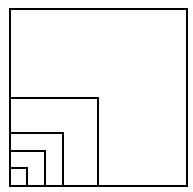
\includegraphics[scale=0.5]{bildoj/variables-carres.png}
\end{center}
\vspace{1cm}
\section{Grafiki ortangulon je longo kaj lar^go difinitaj}
\noindent Oni difinos ^ci tie proceduron nomatan \texttt{ort} kiu
dependu je du variabloj reprezentantaj la du dimensiojn de ortangulo.
\texttt{ort 200 100} grafikos ortangulon je alto $200$ kaj lar^go $100$.
\begin{verbatim}
por ort :lo :la
ripetu 2 [an :lo dn 90 an :la dn 90]
fino
\end{verbatim} 
Faru provojn:
\begin{verbatim}
ort 200 100 ort 100 300 ort 50 150 ort 1 20 ort 100 2 
\end{verbatim}
Kompreneble, se vi donas nur unu argumenton al la proceduro
\texttt{ort}, l' interpretilo signalos per erarmesa^go ke la proceduro
atendas alian argumenton.
\section{Grafiki formon je malsamaj ampleksoj}
\noindent
Ni jam vidis kiel grafiki kvadraton, ortangulon je malsamaj ampleksoj.
Ni reprenos l' ekzemplon de la domo de p.~\pageref{maison} kaj vidos
kiel modifi la kodon por grafiki la domon je la dezirata skalo.

La celo estas pasigi argumenton al proceduro \texttt{domo} por ke la^u
la parametro, la domo estu pli a^u malpli granda.  Ni deziras ke 
\texttt{domo 1} grafiku la domon je reala amplekso.

\texttt{domo 0.5} grafikos domon je skalo $0.5$.

\texttt{domo 2} grafikos domon je dimensioj duoblaj, ktp.

La koncepto proporcieco estas kompreneble subka^sita.  En reala
grando, la proceduro \texttt{kvadrato} estis jena:
\begin{verbatim}
por kvadrato
ripetu 4 [an 150 dn 90]
fino
\end{verbatim}
^Ciuj originalaj diminsioj de la domo estas multiplikitaj per la
skalo.  La proceduro \texttt{kvadrato} esti^gas:
\begin{verbatim}
por kvadrato :l
ripetu 4 [an 150*:l dn 90]
fino
\end{verbatim}
Do kiam oni tajpos \texttt{kvadrato 2}, la kvadrato havos lateron
longan je $150\times2=300$.  La proporciojn oni respektos!  Efektive,
oni rimarku ke necesos repreni ^ciujn procedurojn kaj ^san^gi la
longojn je movo la^u la jena maniero:

\texttt{an 70} fari^gos \texttt{an 70*:l}

\texttt{an 45} fari^gos \texttt{an 45*:l}

ktp.

\begin{verbatim}
por kvadrato :l
ripetu 4 [an 150*:l dn 90]
fino

por tri :l
ripetu 3[an 150*:l dn 120]
fino

por pordo :l
ripetu 2 [an 70*:l dn 90 an 50*:l dn 90]
fino

por kam :l
an 55*:l dn 90 an 20*:l dn 90 an 20*:l
fino

por mov1 :l
dn 90 an 50*:l mdn 90
fino

por mov2 :l
mdn 90 an 50*:l dn 90 an 150*:l dn 30
fino

por mov3 :l
l dn 60 an 20*:l mdn 90 an 35*:l ml
fino

por dom :l
kvadrato :l mov1 :l pordo :l mov2 :l tri :l mov3 :l kam :l
fino
\end{verbatim}

\section{Ekzerco:}
\noindent Realigu la desegnojn jenajn per variabloj tiel ke oni povas
obteni ilin je diversaj ampleksoj.

\begin{center}
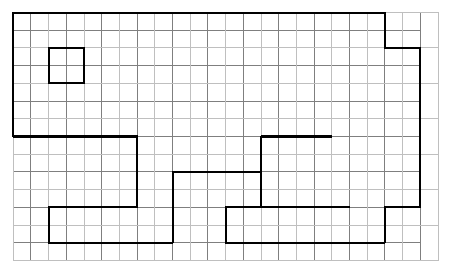
\includegraphics[scale=0.7]{bildoj/variables-grenouille.png}
\end{center}
\begin{center}
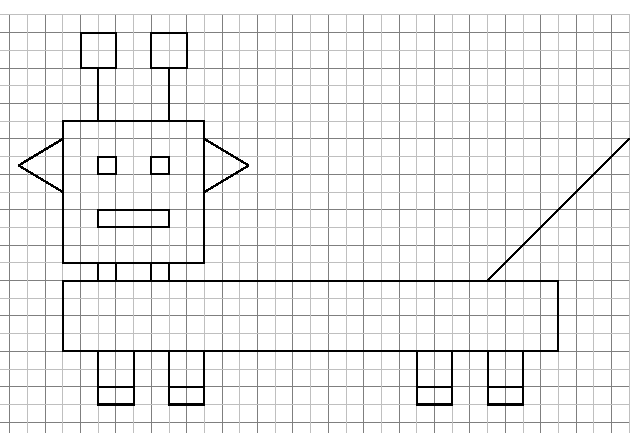
\includegraphics[scale=0.75]{bildoj/variables-robot.png}
\end{center}
